\documentclass[aspectratio=169,10pt]{beamer}
\usepackage{amssymb}
\usepackage[T1]{fontenc}
\usepackage{amsmath,amssymb,amsthm}
\usepackage{graphicx}
\usepackage{listings}
\usepackage{xcolor}
\usepackage{tikz}
\usetikzlibrary{positioning,matrix,arrows.meta}
\usetikzlibrary{calc}
\usepackage{algorithm}
\usepackage{algorithmic}
\usepackage{hyperref}
\usepackage{mimic}
\usepackage{adjustbox} 
% Theme settings
\usetheme{Madrid}
\usecolortheme{seahorse}
\setbeamertemplate{navigation symbols}{}
\setbeamertemplate{footline}[frame number]

% Code listing configuration
\lstset{
    language=Python,
    basicstyle=\ttfamily\scriptsize,
    keywordstyle=\color{blue}\bfseries,
    stringstyle=\color{red},
    commentstyle=\color{green!60!black},
    showstringspaces=false,
    breaklines=true,
    breakatwhitespace=true,
    frame=single,
    numbers=left,
    numberstyle=\tiny\color{gray},
    xleftmargin=1em,
    framexleftmargin=1em
}

% Title page information
\title{Reinforcement Learning}
\subtitle{Lecture 6: Deep Q-Networks (DQN)}
\author{Taehoon Kim}
\institute{Sogang University MIMIC Lab \\ \url{https://mimic-lab.com}}
\date{Fall Semester 2025}


\begin{document}

% Slide 1: Title
\frame{\titlepage}


% Slide 3: Session Goals
\begin{frame}{Session Goals}
\textbf{By the end of this lecture, you will be able to:}
\begin{enumerate}
    \item Explain why tabular Q-learning fails with high-dimensional state spaces
    \item Understand how DQN addresses divergence risks with experience replay and target networks
    \item Derive the DQN learning target and implement the Huber loss objective
    \item Implement a production-grade DQN agent in PyTorch with:
    \begin{itemize}
        \item Replay buffer, target network, and $\epsilon$-greedy exploration
        \item Mixed precision (AMP) and torch.compile() acceleration
        \item Checkpoint save/restore and TensorBoard logging
    \end{itemize}
    \item Run ablations on hyperparameters and interpret results
\end{enumerate}

\vspace{0.3cm}
\textbf{Prerequisites:} Q-learning (Lecture 5), PyTorch basics (Lecture 2)
\end{frame}

% Slide 4: Section 1 - Theory Foundations
\begin{frame}{Foundations Overview}
\textbf{Focus to kick things off}
\begin{itemize}
    \item Diagnose why tabular Q-learning breaks in large/continuous spaces
    \item Build up the DQN recipe: replay buffer, target network, loss
    \item Reason about stability tricks (Double DQN, Huber loss, AMP)
\end{itemize}

\vspace{0.3cm}
\textbf{Flow}
\begin{enumerate}
    \item Revisiting tabular Q-learning pitfalls
    \item Introducing neural function approximation
    \item Deriving the DQN update and variants
\end{enumerate}

\vspace{0.3cm}
\textbf{Goal:} Bridge tabular intuition to deep RL foundations before coding.
\end{frame}

% Slide 5: The Curse of Dimensionality
\begin{frame}{The Curse of Dimensionality}
\textbf{Tabular Q-Learning Limitations:}
\begin{itemize}
    \item State space explosion: CartPole with 10 bins/dimension $\rightarrow 10^4 = 10,000$ states
    \item Memory requirements: $O(|S| \times |A|)$
    \item No generalization between similar states
    \item Must visit every state-action pair
\end{itemize}

\vspace{0.3cm}
\textbf{Real-world Examples:}
\begin{itemize}
    \item Atari games: $210 \times 160$ pixels $\times$ 128 colors $\approx 10^{120,000}$ states
    \item Robotics: Continuous joint angles and velocities
    \item Autonomous driving: High-dimensional sensor inputs
\end{itemize}

\vspace{0.3cm}
\alert{Solution: Function Approximation with Neural Networks}

% Slide 6: Function Approximation
\end{frame}
\begin{frame}{Function Approximation in Q-Learning}
\textbf{From Table to Function:}
\begin{columns}[T]
\begin{column}{0.5\textwidth}
\textbf{Tabular Q-Learning:}
\begin{itemize}
    \item $Q: S \times A \rightarrow \mathbb{R}$
    \item Stored as table $Q[s,a]$
    \item Update: $Q[s,a] \leftarrow$ target
    \item Exact values per state
\end{itemize}
\end{column}
\begin{column}{0.5\textwidth}
\textbf{Deep Q-Learning:}
\begin{itemize}
    \item $Q_\theta: S \times A \rightarrow \mathbb{R}$
    \item Neural network with parameters $\theta$
    \item Update: $\theta \leftarrow \theta - \alpha \nabla_\theta L$
    \item Approximate values
\end{itemize}
\end{column}
\end{columns}

\vspace{0.5cm}
\textbf{Benefits of Neural Networks:}
\begin{itemize}
    \item Automatic feature extraction
    \item Generalization to similar states
    \item Handles high-dimensional inputs (images, etc.)
    \item Compact representation
\end{itemize}
\end{frame}

% Slide 7: The Naive Approach Fails
\begin{frame}{Why Naive Neural Q-Learning Fails}
\textbf{Deadly Triad of Instability:}
\begin{enumerate}
    \item \textbf{Function Approximation}: Non-tabular representation
    \item \textbf{Bootstrapping}: Using estimates to update estimates
    \item \textbf{Off-policy Learning}: Learning from old experiences
\end{enumerate}

\vspace{0.3cm}
\textbf{Specific Problems:}
\begin{itemize}
    \item \textbf{Moving Targets}: $Q_\theta(s',a')$ changes as we update $\theta$
    \item \textbf{Correlation}: Sequential samples are highly correlated
    \item \textbf{Feedback Loops}: Updates affect future targets
    \item \textbf{Overestimation}: Max operator causes positive bias
\end{itemize}

\vspace{0.3cm}
\alert{Result: Divergence, oscillation, or poor performance}

% Slide 8: DQN Innovation 1 - Experience Replay
\end{frame}
\begin{frame}[fragile]{DQN Innovation 1: Experience Replay}
\textbf{Breaking Correlation with Memory:}
\begin{itemize}
    \item Store transitions $(s, a, r, s', done)$ in replay buffer $\mathcal{D}$
    \item Sample random mini-batches for training
    \item Breaks temporal correlation
    \item Improves sample efficiency (reuse experiences)
\end{itemize}

\vspace{0.3cm}
\textbf{Replay Buffer Implementation:}
\begin{lstlisting}
class ReplayBuffer:
    def __init__(self, capacity):
        self.buffer = deque(maxlen=capacity)
    
    def push(self, state, action, reward, next_state, done):
        self.buffer.append((state, action, reward, next_state, done))
    
    def sample(self, batch_size):
        return random.sample(self.buffer, batch_size)
\end{lstlisting}

% Slide 9: Experience Replay Benefits
\end{frame}
\begin{frame}{Experience Replay: Why It Works}
\begin{columns}[T]
\begin{column}{0.5\textwidth}
\textbf{Without Replay:}
\begin{itemize}
    \item Samples: $s_t, s_{t+1}, s_{t+2}, ...$
    \item High correlation
    \item Recent bias
    \item Catastrophic forgetting
    \item Unstable gradients
\end{itemize}
\end{column}
\begin{column}{0.5\textwidth}
\textbf{With Replay:}
\begin{itemize}
    \item Samples: $s_{17}, s_{203}, s_{5}, ...$
    \item I.I.D.-like sampling
    \item Balanced experience
    \item Better coverage
    \item Stable gradients
\end{itemize}
\end{column}
\end{columns}

\vspace{0.5cm}
\textbf{Key Parameters:}
\begin{itemize}
    \item Buffer size: Typically $10^4$ to $10^6$ transitions
    \item Batch size: Usually 32-256
    \item Start learning after: 1000+ transitions (warmup)
\end{itemize}

% Slide 10: DQN Innovation 2 - Target Network
\end{frame}
\begin{frame}{DQN Innovation 2: Target Network}
\textbf{Stabilizing the Learning Target:}
\begin{itemize}
    \item Maintain two networks: Online $Q_\theta$ and Target $Q_{\theta^-}$
    \item Use target network for computing TD targets
    \item Update target network periodically (every $C$ steps)
\end{itemize}

\vspace{0.3cm}
\textbf{The Key Insight:}
\begin{align}
\text{Without target network:} & \quad y = r + \gamma \max_{a'} Q_\theta(s', a') \\
\text{With target network:} & \quad y = r + \gamma \max_{a'} Q_{\theta^-}(s', a')
\end{align}

Target $\theta^-$ remains fixed during updates, breaking harmful feedback loops!

\vspace{0.3cm}
\textbf{Update Strategies:}
\begin{itemize}
    \item Hard update: $\theta^- \leftarrow \theta$ every $C$ steps
    \item Soft update: $\theta^- \leftarrow \tau\theta + (1-\tau)\theta^-$ each step
\end{itemize}

\end{frame}

\begin{frame}{Target Network Flow Forward}
\begin{center}
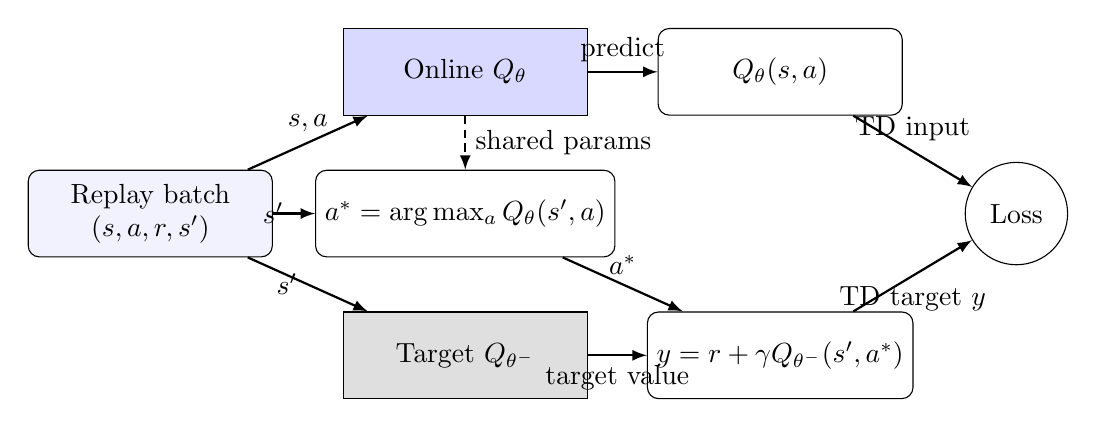
\begin{tikzpicture}[>=latex]
    \tikzset{
        block/.style={draw, rounded corners, minimum width=3.1cm, minimum height=1.1cm, align=center},
        module/.style={draw, rectangle, minimum width=3.1cm, minimum height=1.1cm, align=center},
        flow/.style={->, thick},
        dashedflow/.style={->, thick, densely dashed}
    }

    \node[block, fill=blue!5] (batch) at (0,0) {Replay batch\\$(s,a,r,s')$};
    \node[module, fill=blue!15] (online) at (4.0,1.8) {Online $Q_{\theta}$};
    \node[module, fill=gray!25] (target) at (4.0,-1.8) {Target $Q_{\theta^-}$};

    \node[block] (qpred) at (8.0,1.8) {$Q_{\theta}(s,a)$};
    \node[block] (astar) at (4.0,0.0) {$a^* = \arg\max_a Q_{\theta}(s',a)$};
    \node[block] (yvalue) at (8.0,-1.8) {$y = r + \gamma Q_{\theta^-}(s',a^*)$};
    \node[draw, circle, minimum size=1.3cm, align=center] (loss) at (11.0,0.0) {Loss};

    \draw[flow] (batch) -- node[above] {$s,a$} (online);
    \draw[flow] (online) -- node[above] {predict} (qpred);
    \draw[flow] (qpred) -- node[above] {TD input} (loss);

    \draw[flow] (batch) -- node[left] {$s'$} (astar);
    \draw[dashedflow] (online) -- node[right] {shared params} (astar);
    \draw[flow] (astar) -- node[above] {$a^*$} (yvalue);

    \draw[flow] (batch) -- node[left] {$s'$} (target);
    \draw[flow] (target) -- node[below] {target value} (yvalue);
    \draw[flow] (yvalue) -- node[below] {TD target $y$} (loss);
\end{tikzpicture}
\end{center}

\textbf{Forward pass:}
\begin{enumerate}
    \item Sample a mini-batch from replay to evaluate $Q_{\theta}(s,a)$.
    \item Use the online network to select $a^*$ for each next state $s'$.
    \item Combine $a^*$ with the frozen target network to construct TD targets $y$.
\end{enumerate}

\end{frame}

\begin{frame}{Target Network Flow Updates}
\begin{center}
\begin{adjustbox}{max width=\linewidth}
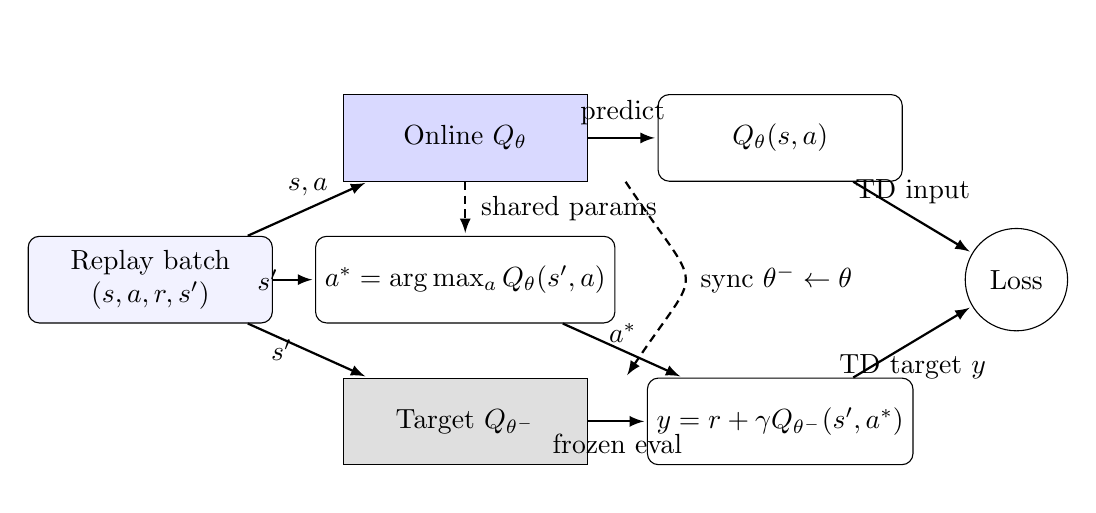
\begin{tikzpicture}[
    >=latex,
    block/.style={draw, rounded corners, minimum width=3.1cm, minimum height=1.1cm, align=center},
    module/.style={draw, rectangle, minimum width=3.1cm, minimum height=1.1cm, align=center},
    flow/.style={->, thick, shorten >=1pt},
    dashedflow/.style={->, thick, densely dashed, shorten >=1pt},
    grad/.style={->, very thick, red, shorten >=1pt},
    stopgrad/.style={-|, very thick, red, shorten >=1pt}
]

\node[block, fill=blue!5] (batch) at (0,0) {Replay batch\\$(s,a,r,s')$};
\node[module, fill=blue!15] (online) at (4.0,1.8) {Online $Q_{\theta}$};
\node[module, fill=gray!25] (target) at (4.0,-1.8) {Target $Q_{\theta^-}$};

\node[block] (qpred) at (8.0,1.8) {$Q_{\theta}(s,a)$};
\node[block] (astar) at (4.0,0.0) {$a^* = \arg\max_a Q_{\theta}(s',a)$};
\node[block] (yvalue) at (8.0,-1.8) {$y = r + \gamma Q_{\theta^-}(s',a^*)$};
\node[draw, circle, minimum size=1.3cm, align=center, inner sep=1pt] (loss) at (11.0,0.0) {Loss};

% forward flows
\draw[flow] (batch) -- node[above, yshift=1pt] {$s,a$} (online);
\draw[flow] (online) -- node[above, yshift=1pt] {predict} (qpred);
\draw[flow] (qpred) -- node[above, yshift=1pt] {TD input} (loss);

\draw[flow] (batch) -- node[left, xshift=-2pt] {$s'$} (astar);
\draw[dashedflow] (online) -- node[right, xshift=2pt] {shared params} (astar);
\draw[flow] (astar) -- node[above, yshift=-1pt] {$a^*$} (yvalue);

\draw[flow] (batch) -- node[left, xshift=-2pt] {$s'$} (target);
\draw[flow] (target) -- node[below, yshift=-1pt] {frozen eval} (yvalue);
\draw[flow] (yvalue) -- node[below, yshift=-1pt] {TD target $y$} (loss);

\draw[dashedflow]
  ([xshift=0.48cm]online.south east)
   .. controls +(1.0,-1.5) and +(1.0,1.5) ..
   node[right, xshift=2pt] {sync $\theta^- \leftarrow \theta$}
   ([xshift=0.48cm]target.north east);

\path[use as bounding box] (-0.8,-2.6) rectangle (11.6,3.2);

\end{tikzpicture}
\end{adjustbox}
\end{center}

\vspace{0.2cm}
Updates and stability:
\begin{enumerate}
    \item Backpropagate the loss through $Q_{\theta}$ only. Keep $Q_{\theta^-}$ frozen.
    \item Periodically copy parameters $\left(\theta^- \leftarrow \theta\right)$ to refresh the target.
\end{enumerate}
\end{frame}

\begin{frame}{DQN Loss Function}
\textbf{The DQN Objective:}
\begin{align}
L(\theta) = \mathbb{E}_{(s,a,r,s') \sim \mathcal{D}} \left[ \left( y - Q_\theta(s,a) \right)^2 \right]
\end{align}

where the target is:
\begin{align}
y = r + \gamma (1 - done) \cdot \max_{a'} Q_{\theta^-}(s', a')
\end{align}

\vspace{0.3cm}
\textbf{Huber Loss (Smooth L1):}
\begin{align}
\mathcal{L}_\delta(x) = \begin{cases}
\frac{1}{2}x^2 & \text{if } |x| \leq \delta \\
\delta(|x| - \frac{1}{2}\delta) & \text{otherwise}
\end{cases}
\end{align}

\textbf{Benefits:} Less sensitive to outliers, prevents gradient explosion
\end{frame}

% Slide 13: Complete DQN Algorithm
\begin{frame}{The Complete DQN Algorithm}
\begin{algorithmic}[1]
\STATE Initialize replay buffer $\mathcal{D}$ with capacity $N$
\STATE Initialize Q-network $Q_\theta$ with random weights
\STATE Initialize target network $Q_{\theta^-}$ with $\theta^- = \theta$
\FOR{episode = 1 to $M$}
    \STATE Initialize state $s_1$
    \FOR{$t = 1$ to $T$}
        \STATE Select action $a_t = \begin{cases}
            \text{random action} & \text{with probability } \epsilon \\
            \arg\max_a Q_\theta(s_t, a) & \text{otherwise}
        \end{cases}$
        \STATE Execute $a_t$, observe $r_t$, $s_{t+1}$
        \STATE Store $(s_t, a_t, r_t, s_{t+1})$ in $\mathcal{D}$
        \STATE Sample mini-batch from $\mathcal{D}$
        \STATE Compute targets $y_i = r_i + \gamma \max_{a'} Q_{\theta^-}(s'_i, a')$
        \STATE Update $\theta$ by minimizing $L = \frac{1}{|B|}\sum_i (y_i - Q_\theta(s_i, a_i))^2$
        \STATE Every $C$ steps: $\theta^- \leftarrow \theta$
    \ENDFOR
\ENDFOR
\end{algorithmic}

% Slide 14: Double DQN
\end{frame}
\begin{frame}{Double DQN: Reducing Overestimation}
\textbf{The Overestimation Problem:}
\begin{itemize}
    \item Max operator in Q-learning causes positive bias
    \item $\mathbb{E}[\max_a Q(s,a)] \geq \max_a \mathbb{E}[Q(s,a)]$ (Jensen's inequality)
    \item Errors accumulate through bootstrapping
\end{itemize}

\vspace{0.3cm}
\textbf{Double DQN Solution:}
\begin{itemize}
    \item Decouple action selection from evaluation
    \item Use online network to select actions
    \item Use target network to evaluate them
\end{itemize}

\begin{align}
\text{DQN:} & \quad y = r + \gamma \max_{a'} Q_{\theta^-}(s', a') \\
\text{Double DQN:} & \quad y = r + \gamma Q_{\theta^-}(s', \arg\max_{a'} Q_\theta(s', a'))
\end{align}

% Slide 15: Epsilon-Greedy Exploration
\end{frame}
\begin{frame}[fragile]{Exploration Strategy: $\epsilon$-Greedy}
\textbf{Balancing Exploration and Exploitation:}
\begin{lstlisting}
def select_action(state, epsilon):
    if random.random() < epsilon:
        return env.action_space.sample()  # Explore
    else:
        q_values = q_network(state)
        return q_values.argmax()          # Exploit
\end{lstlisting}

\vspace{0.3cm}
\textbf{Epsilon Scheduling:}
\begin{itemize}
    \item Linear decay: $\epsilon_t = \epsilon_{start} - t \cdot \frac{\epsilon_{start} - \epsilon_{end}}{T}$
    \item Exponential decay: $\epsilon_t = \epsilon_{end} + (\epsilon_{start} - \epsilon_{end}) \cdot e^{-t/\tau}$
    \item Step decay: Reduce by factor at milestones
\end{itemize}

\textbf{Typical values:} $\epsilon_{start} = 1.0$, $\epsilon_{end} = 0.01$
\end{frame}

% Slide 16: Hyperparameters Overview
\begin{frame}{DQN Hyperparameters}
\begin{table}
\small
\begin{tabular}{l|l|l}
\hline
\textbf{Parameter} & \textbf{Typical Value} & \textbf{Description} \\
\hline
Learning rate & $10^{-4}$ to $10^{-3}$ & Gradient descent step size \\
Batch size & 32-256 & Mini-batch size \\
Buffer size & $10^4$ to $10^6$ & Replay buffer capacity \\
Target update & 1000-10000 steps & Hard update frequency \\
$\gamma$ & 0.99 & Discount factor \\
$\epsilon_{start}$ & 1.0 & Initial exploration \\
$\epsilon_{end}$ & 0.01-0.1 & Final exploration \\
Hidden layers & [128, 128] & Network architecture \\
Optimizer & Adam & Gradient optimizer \\
Loss & Huber & Loss function \\
\hline
\end{tabular}
\end{table}
\end{frame}

% Slide 17: Common Pitfalls
\begin{frame}{Common Pitfalls and Solutions}
\begin{enumerate}
    \item \textbf{Insufficient Warmup}
    \begin{itemize}
        \item Problem: Learning from small buffer
        \item Solution: Start after 1000+ transitions
    \end{itemize}
    
    \item \textbf{Exploration Collapse}
    \begin{itemize}
        \item Problem: $\epsilon$ decays too quickly
        \item Solution: Longer decay schedule
    \end{itemize}
    
    \item \textbf{Gradient Explosion}
    \begin{itemize}
        \item Problem: Unstable training
        \item Solution: Gradient clipping, Huber loss
    \end{itemize}
    
    \item \textbf{Reward Scale}
    \begin{itemize}
        \item Problem: Rewards too large/small
        \item Solution: Reward clipping or normalization
    \end{itemize}
    
    \item \textbf{Target Update Frequency}
    \begin{itemize}
        \item Problem: Too frequent or too rare
        \item Solution: Tune based on environment
    \end{itemize}
\end{enumerate}
\end{frame}

% Slide 18: DQN Variants
\begin{frame}{DQN Variants and Extensions}
\textbf{Major DQN Improvements:}
\begin{itemize}
    \item \textbf{Double DQN (2015)}: Reduce overestimation bias
    \item \textbf{Prioritized Replay (2015)}: Sample important transitions more
    \item \textbf{Dueling DQN (2016)}: Separate value and advantage streams
    \item \textbf{Rainbow (2017)}: Combine all improvements
    \item \textbf{C51 (2017)}: Distributional Q-learning
    \item \textbf{Noisy Networks (2017)}: Parameter noise for exploration
\end{itemize}

\vspace{0.3cm}
\textbf{Rainbow Components:}
\begin{enumerate}
    \item Double Q-learning
    \item Prioritized replay
    \item Dueling networks
    \item Multi-step learning
    \item Distributional RL
    \item Noisy networks
\end{enumerate}
\end{frame}

% Slide 19: When to Use DQN
\begin{frame}{When to Use DQN}
\textbf{Good fit for DQN:}
\begin{itemize}
    \item Discrete action spaces
    \item High-dimensional observations (images)
    \item Need sample efficiency
    \item Off-policy learning beneficial
    \item Deterministic environments
\end{itemize}

\vspace{0.3cm}
\textbf{Consider alternatives when:}
\begin{itemize}
    \item Continuous actions $\rightarrow$ DDPG, TD3, SAC
    \item On-policy preferred $\rightarrow$ PPO, A2C
    \item Simple state space $\rightarrow$ Tabular Q-learning
    \item Safety critical $\rightarrow$ Conservative algorithms
\end{itemize}

\vspace{0.3cm}
\textbf{Success stories:} Atari games, resource allocation, trading
\end{frame}

% Slide 20: Mathematical Deep Dive
\begin{frame}{Key Equations for DQN}
\textbf{Bellman Optimality with Function Approximation:}
\begin{align}
Q^*(s,a) = \mathbb{E}_{s'} \left[ r + \gamma \max_{a'} Q^*(s',a') \mid s,a \right]
\end{align}

\textbf{Semi-gradient Update:}
\begin{align}
\theta_{t+1} = \theta_t + \alpha \left[ y_t - Q_\theta(s_t,a_t) \right] \nabla_\theta Q_\theta(s_t,a_t)
\end{align}

\textbf{Convergence Conditions (Tabular):}
\begin{itemize}
    \item All state-action pairs visited infinitely
    \item Learning rate satisfies Robbins-Monro conditions
    \item $\sum_t \alpha_t = \infty$, $\sum_t \alpha_t^2 < \infty$
\end{itemize}

\alert{Note: Neural Q-learning convergence not guaranteed!}
\end{frame}


% Slide 24: Replay Buffer Implementation
\begin{frame}[fragile]{Efficient Replay Buffer}
\begin{lstlisting}
class ReplayBuffer:
    def __init__(self, capacity, obs_dim):
        # Pre-allocate arrays for efficiency
        self.observations = np.zeros((capacity, obs_dim), 
                                    dtype=np.float32)
        self.actions = np.zeros(capacity, dtype=np.int64)
        self.rewards = np.zeros(capacity, dtype=np.float32)
        self.next_observations = np.zeros((capacity, obs_dim), 
                                         dtype=np.float32)
        self.dones = np.zeros(capacity, dtype=np.float32)
        
        self.position = 0
        self.size = 0
        self.capacity = capacity
    
    def push(self, obs, action, reward, next_obs, done):
        idx = self.position
        self.observations[idx] = obs
        self.actions[idx] = action
        # ... store other components
        self.position = (self.position + 1) % self.capacity
        self.size = min(self.size + 1, self.capacity)
\end{lstlisting}

% Slide 25: Q-Network Architecture
\end{frame}
\begin{frame}[fragile]{Q-Network Implementation}
\begin{lstlisting}
class QNetwork(nn.Module):
    def __init__(self, obs_dim, n_actions, 
                 hidden_sizes=(128, 128)):
        super().__init__()
        
        layers = []
        input_size = obs_dim
        
        # Build hidden layers
        for hidden_size in hidden_sizes:
            layers.append(nn.Linear(input_size, hidden_size))
            layers.append(nn.ReLU())
            input_size = hidden_size
        
        # Output layer (Q-values for each action)
        layers.append(nn.Linear(input_size, n_actions))
        
        self.network = nn.Sequential(*layers)
    
    def forward(self, x):
        return self.network(x)  # Shape: [batch_size, n_actions]
\end{lstlisting}
\end{frame}

% Slide 26: Target Network Updates
\begin{frame}[fragile]{Target Network Mechanism}
\begin{lstlisting}
def hard_update(target_net, online_net):
    """Copy weights from online to target network"""
    target_net.load_state_dict(online_net.state_dict())

def soft_update(target_net, online_net, tau=0.005):
    """Polyak averaging update"""
    with torch.no_grad():
        for target_param, param in zip(
            target_net.parameters(), 
            online_net.parameters()
        ):
            target_param.data.copy_(
                tau * param.data + (1 - tau) * target_param.data
            )

# Usage in training loop
if step % target_update_freq == 0:
    hard_update(target_network, q_network)
# OR for soft updates:
soft_update(target_network, q_network, tau=0.005)
\end{lstlisting}
\end{frame}

% Slide 27: Computing DQN Loss
\begin{frame}[fragile]{DQN Loss Computation}
\begin{lstlisting}
def compute_dqn_loss(batch, q_network, target_network, 
                     gamma=0.99):
    obs, actions, rewards, next_obs, dones = batch
    
    # Current Q-values for taken actions
    q_values = q_network(obs)  # [B, n_actions]
    q_values = q_values.gather(1, actions.unsqueeze(1))
    q_values = q_values.squeeze()  # [B]
    
    # Compute targets with target network
    with torch.no_grad():
        next_q_values = target_network(next_obs)  # [B, n_actions]
        next_q_max = next_q_values.max(1)[0]  # [B]
        
        # TD targets
        targets = rewards + gamma * (1 - dones) * next_q_max
    
    # Huber loss
    loss = F.huber_loss(q_values, targets)
    return loss
\end{lstlisting}
\end{frame}

% Slide 28: Double DQN Implementation
\begin{frame}[fragile]{Double DQN: Reducing Overestimation}
\begin{lstlisting}
def compute_double_dqn_loss(batch, q_network, target_network, 
                           gamma=0.99):
    obs, actions, rewards, next_obs, dones = batch
    
    # Current Q-values
    q_values = q_network(obs).gather(1, actions.unsqueeze(1))
    q_values = q_values.squeeze()
    
    with torch.no_grad():
        # Action selection with online network
        next_q_online = q_network(next_obs)
        next_actions = next_q_online.argmax(1, keepdim=True)
        
        # Action evaluation with target network
        next_q_target = target_network(next_obs)
        next_q_values = next_q_target.gather(1, next_actions)
        next_q_values = next_q_values.squeeze()
        
        targets = rewards + gamma * (1 - dones) * next_q_values

    return F.huber_loss(q_values, targets)
\end{lstlisting}
\end{frame}

% Slide 29: Training Loop
\begin{frame}[fragile]{Main Training Loop}
\begin{lstlisting}
def train_dqn(env, n_episodes=1000):
    q_network = QNetwork(obs_dim, n_actions).to(device)
    target_network = QNetwork(obs_dim, n_actions).to(device)
    target_network.load_state_dict(q_network.state_dict())
    
    optimizer = optim.Adam(q_network.parameters(), lr=1e-3)
    buffer = ReplayBuffer(capacity=10000, obs_dim=obs_dim)
    
    for episode in range(n_episodes):
        obs, _ = env.reset()
        episode_reward = 0
        
        while not done:
            # Select action (epsilon-greedy)
            action = select_action(obs, epsilon)
            next_obs, reward, done, _, _ = env.step(action)
            
            # Store and learn
            buffer.push(obs, action, reward, next_obs, done)
            if len(buffer) >= batch_size:
                batch = buffer.sample(batch_size)
                loss = compute_dqn_loss(batch, q_network, 
                                       target_network)
                # ... optimize
\end{lstlisting}
\end{frame}



% Slide 31: Logging and Monitoring
\begin{frame}[fragile]{TensorBoard Integration}
\begin{lstlisting}
from torch.utils.tensorboard import SummaryWriter

writer = SummaryWriter('runs/dqn_experiment')

# Log scalars
writer.add_scalar('loss/td_error', loss.item(), step)
writer.add_scalar('metrics/episode_reward', reward, episode)
writer.add_scalar('metrics/epsilon', epsilon, step)

# Log hyperparameters and metrics
writer.add_hparams(
    {'lr': 1e-3, 'batch_size': 32, 'gamma': 0.99},
    {'final_reward': best_reward}
)

# Visualize in terminal:
# tensorboard --logdir runs/
\end{lstlisting}

\textbf{Key Metrics to Track:}
Loss, episode rewards, Q-values, epsilon, learning rate
\end{frame}

% Slide 32: Checkpointing
\begin{frame}[fragile]{Saving and Loading Models}
\begin{lstlisting}
def save_checkpoint(agent, filepath):
    checkpoint = {
        'q_network': agent.q_network.state_dict(),
        'target_network': agent.target_network.state_dict(),
        'optimizer': agent.optimizer.state_dict(),
        'episode': agent.episode,
        'epsilon': agent.epsilon,
        'replay_buffer': agent.buffer,  # Optional
        'config': agent.config
    }
    torch.save(checkpoint, filepath)

def load_checkpoint(filepath):
    checkpoint = torch.load(filepath, map_location=device)
    
    agent.q_network.load_state_dict(checkpoint['q_network'])
    agent.target_network.load_state_dict(
        checkpoint['target_network'])
    agent.optimizer.load_state_dict(checkpoint['optimizer'])
    # ... restore other components
    
    return checkpoint['episode']
\end{lstlisting}
\end{frame}

% Slide 33: Evaluation Protocol
\begin{frame}[fragile]{Proper Evaluation}
\begin{lstlisting}
def evaluate(agent, env, n_episodes=10):
    """Evaluate agent without exploration"""
    eval_rewards = []
    
    for episode in range(n_episodes):
        obs, _ = env.reset(seed=seed + episode)
        episode_reward = 0
        done = False
        
        while not done:
            # Greedy action selection (no exploration)
            with torch.no_grad():
                q_values = agent.q_network(
                    torch.FloatTensor(obs).unsqueeze(0))
                action = q_values.argmax().item()
            
            obs, reward, terminated, truncated, _ = env.step(action)
            done = terminated or truncated
            episode_reward += reward
        
        eval_rewards.append(episode_reward)
    
    return np.mean(eval_rewards), np.std(eval_rewards)
\end{lstlisting}
\end{frame}

% Slide 34: Hyperparameter Tuning
\begin{frame}[fragile]{Hyperparameter Tuning Strategy}
\textbf{Grid Search Example:}
\begin{lstlisting}
param_grid = {
    'lr': [1e-3, 3e-4, 1e-4],
    'batch_size': [32, 64, 128],
    'target_update': [100, 500, 1000],
    'buffer_size': [10000, 50000]
}
\end{lstlisting}

\textbf{Important Relationships:}
\begin{itemize}
    \item Larger buffer $\rightarrow$ more stable but slower
    \item Frequent target updates $\rightarrow$ less stable
    \item Larger batch $\rightarrow$ more stable gradients
    \item Higher $\gamma$ $\rightarrow$ longer-term planning
\end{itemize}

\textbf{Start with:}
\begin{itemize}
    \item Published hyperparameters for similar tasks
    \item Conservative values (small LR, large buffer)
    \item Tune one parameter at a time
\end{itemize}
\end{frame}

% Slide 35: Debugging DQN
\begin{frame}{Debugging Checklist}
\textbf{Common Issues and Solutions:}
\begin{enumerate}
    \item \textbf{Q-values exploding}
    \begin{itemize}
        \item Check reward scale
        \item Verify target network updates
        \item Use gradient clipping
    \end{itemize}
    
    \item \textbf{No learning progress}
    \begin{itemize}
        \item Increase exploration ($\epsilon$)
        \item Check replay buffer filling
        \item Verify loss computation
    \end{itemize}
    
    \item \textbf{Unstable training}
    \begin{itemize}
        \item Reduce learning rate
        \item Increase batch size
        \item Use Huber loss instead of MSE
    \end{itemize}
    
    \item \textbf{Poor final performance}
    \begin{itemize}
        \item Tune exploration schedule
        \item Increase network capacity
        \item Try Double DQN
    \end{itemize}
\end{enumerate}
\end{frame}

% Slide 36: CartPole Results
\begin{frame}{Expected Results: CartPole-v1}
\textbf{Training Progression:}
\begin{itemize}
    \item Episodes 1-50: Random behavior (reward $\approx$ 20)
    \item Episodes 50-100: Learning begins (reward $\approx$ 50-100)
    \item Episodes 100-150: Rapid improvement (reward $\approx$ 150-200)
    \item Episodes 150+: Solved (reward = 500, maximum)
\end{itemize}

\vspace{0.3cm}
\textbf{Typical Training Curve:}
\begin{center}
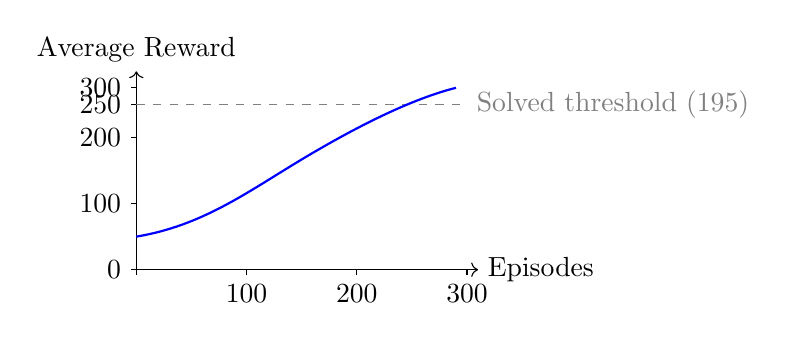
\begin{tikzpicture}[scale=0.7]
    \draw[->] (0,0) -- (6.2,0) node[right]{Episodes};
    \draw[->] (0,0) -- (0,3.6) node[above]{Average Reward};
    \draw[dashed,gray] (0,3.0) -- (6.0,3.0) node[right]{Solved threshold (195)};
    \draw[thick,blue] (0,0.6) .. controls (1.2,0.8) and (2.0,1.4) .. (3.0,2.0) .. controls (4.0,2.6) and (5.0,3.1) .. (5.8,3.3);
    \draw (0,0) -- (-0.1,0) node[left]{0};
    \draw (0,1.2) -- (-0.1,1.2) node[left]{100};
    \draw (0,2.4) -- (-0.1,2.4) node[left]{200};
    \draw (0,3.0) -- (-0.1,3.0) node[left]{250};
    \draw (0,3.3) -- (-0.1,3.3) node[left]{300};
    \draw (0,0) -- (0,-0.1);
    \draw (2,0) -- (2,-0.1) node[below]{100};
    \draw (4,0) -- (4,-0.1) node[below]{200};
    \draw (6,0) -- (6,-0.1) node[below]{300};
\end{tikzpicture}
\end{center}

\end{frame}

% Slide 37: Ablation Studies
\begin{frame}{Ablation Studies}
\textbf{Component Impact Analysis:}
\begin{table}
\small
\begin{tabular}{l|c|c}
\hline
\textbf{Configuration} & \textbf{Episodes to Solve} & \textbf{Final Reward} \\
\hline
Full DQN & 150 & 500 \\
No target network & Diverges & N/A \\
No replay buffer & 300+ & 200 \\
Small buffer (1000) & 250 & 450 \\
No exploration decay & 400+ & 300 \\
MSE loss (not Huber) & 200 & 480 \\
Double DQN & 130 & 500 \\
\hline
\end{tabular}
\end{table}

\vspace{0.3cm}
\textbf{Key Insights:}
\begin{itemize}
    \item Target network is essential for stability
    \item Replay buffer significantly improves efficiency
    \item Proper exploration schedule crucial
    \item Double DQN provides modest improvement
\end{itemize}
\end{frame}

% Slide 39: Real-world Applications
\begin{frame}{Real-world DQN Applications}
\textbf{Game Playing:}
\begin{itemize}
    \item Atari 2600 games (original DQN paper)
    \item StarCraft II micro-management
    \item Poker and card games
\end{itemize}

\textbf{Robotics:}
\begin{itemize}
    \item Robotic grasping
    \item Navigation in discrete spaces
    \item Task scheduling
\end{itemize}

\textbf{Resource Management:}
\begin{itemize}
    \item Data center cooling (Google)
    \item Network routing
    \item Inventory management
\end{itemize}

\textbf{Finance:}
\begin{itemize}
    \item Portfolio optimization
    \item Trading strategies
    \item Risk management
\end{itemize}
\end{frame}

% Slide 40: Performance Tips
\begin{frame}{Performance Optimization Tips}
\textbf{Memory Efficiency:}
\begin{itemize}
    \item Use numpy arrays in replay buffer
    \item Store observations as uint8 if possible
    \item Implement circular buffer
    \item Clear gradients with \texttt{set\_to\_none=True}
\end{itemize}

\textbf{Computation Speed:}
\begin{itemize}
    \item Batch environment steps (vectorized envs)
    \item Use torch.compile() for JIT optimization
    \item Enable AMP on compatible GPUs
    \item Profile with torch.profiler
\end{itemize}

\textbf{Training Stability:}
\begin{itemize}
    \item Normalize observations
    \item Clip rewards to [-1, 1] range
    \item Use learning rate scheduling
    \item Monitor gradient norms
\end{itemize}
\end{frame}

% Slide 42: Key Mathematical Results
\begin{frame}{Key Mathematical Results}
\textbf{TD Error:}
\begin{align}
\delta_t = r_t + \gamma \max_{a'} Q_{\theta^-}(s_{t+1}, a') - Q_\theta(s_t, a_t)
\end{align}

\textbf{Gradient Update:}
\begin{align}
\theta_{t+1} = \theta_t - \alpha \nabla_\theta L(\theta_t)
\end{align}

\textbf{Loss Gradient:}
\begin{align}
\nabla_\theta L = -\mathbb{E}_{(s,a,r,s') \sim \mathcal{D}} \left[ \delta_t \nabla_\theta Q_\theta(s,a) \right]
\end{align}

\textbf{Optimal Q-function satisfies:}
\begin{align}
Q^*(s,a) = \max_\pi Q^\pi(s,a) \quad \forall s,a
\end{align}
\end{frame}

% Slide 45: Summary of Theory
\begin{frame}{Summary}
\textbf{Key Theoretical Contributions:}
\begin{enumerate}
    \item \textbf{Problem:} Q-learning fails with function approximation
    \item \textbf{Solution 1:} Experience replay breaks correlation
    \item \textbf{Solution 2:} Target network stabilizes learning
    \item \textbf{Enhancement:} Double DQN reduces overestimation
\end{enumerate}

\vspace{0.3cm}
\textbf{Mathematical Foundation:}
\begin{itemize}
    \item Semi-gradient TD learning
    \item Bellman optimality with approximation
    \item Convergence not guaranteed but works in practice
\end{itemize}

\vspace{0.3cm}
\textbf{Critical Insights:}
\begin{itemize}
    \item Deadly triad: FA + bootstrapping + off-policy
    \item Replay enables i.i.d. sampling assumption
    \item Target network breaks feedback loops
\end{itemize}
\end{frame}

\end{document}
